\section{In-context learning performance} \label{sec:icl-performance}

We first investigated how effectively frontier LLMs could generate linguistically grounded mnemonics through in-context learning. This exploration aimed to establish baseline performance and identify optimal prompting strategies before progressing to more resource-intensive approaches.

\subsection{Experimental setup}
We compared different in-context learning approaches to understand how they affect mnemonic generation quality. Using a test set of 50 vocabulary words from SAT and TOEFL exams, we evaluated four distinct prompting strategies with \xteachermodel (multimodal) and \teachermodel (reasoning) \citep{DeepSeek-AIDEEPSEEKR12025,DeepSeekV32025}.

Given a vocabulary \vocab and a list of mnemonic characteristics (\Cref{fig:good-bad-mnemonics}), we designed a prompt $p$ and prompted the model $M$ to generate a \lgm \mnem for \vocab. We repeated this process for 50 vocabulary \vocab, 4 prompts $p$, and 2 models $M$, resulting in 400 total API requests. The prompts were designed to elicit different levels of linguistic reasoning and mnemonic generation strategies, with full description in \Cref{app:prompt-usage}. We used \verb|curator| \citep{BespokeLabBESPOKE2025} with \verb|litellm| orchestration layer to standardize API calls, manage rate limits, and handle retries across experiments.

We evaluated the outputs based on two criteria: \numlist{1} lingusitic grounding, whether there is at least one of the linguistic features (\Cref{tab:linguistic-features}) and \numlist{2} overall quality, which we manually assessed using the given rubric (\Cref{fig:good-bad-mnemonics}).

\subsection{Results} \label{sec:icl-results}

\begin{figure}[htb]
  \centering
  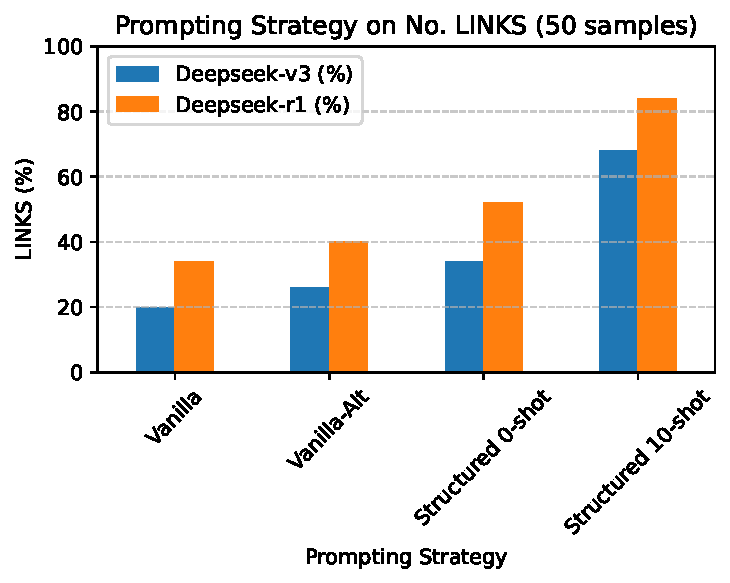
\includegraphics[width=\linewidth]{figures/prompt_comparison.pdf}
  \caption{Comparison of prompting methods (details in \Cref{app:prompt-usage}). Y-axis shows percentage of linguistically-grounded mnemonics generated out of 50 requests for each prompt type.}
  \label{fig:prompting-methods}
\end{figure}

As shown in \Cref{fig:prompting-methods}, we observed significant variation in the linguistic grounding of generated mnemonics based solely on prompt formulation. The vanilla prompt, which simply requested a \lgm for a vocabulary \vocab, produced only 28\% linguistically grounded outputs in only 28\% of cases. Interestingly, changing the terminology from "mnemonic" to "memory cue" increased the proportion of linguistically grounded responses to 42\%, suggesting that the term "mnemonic" may carry pre-training biases that associate it primarily with acronyms or simple keyword methods rather than deeper linguistic analysis \citep{hackmannWordImportanceExplains2024}.

The structured prompt, which explicitly requested a "linguistically grounded mnemonic" and specified that linguistic features should be used, achieved 64\% linguistically grounded outputs. This aligns with findings from \citet{yinDidYouRead2023} that explicit task instructions significantly impact LLM performance.

Most notably, the 10-shot chain-of-thought (CoT) prompt, which included examples of step-by-step linguistic analysis before mnemonic generation, achieved 86\% linguistically grounded responses. This substantial improvement demonstrates that CoT prompting effectively elicits linguistic reasoning capabilities from LLMs \citep{weiChainofThoughtPromptingElicits2022}.

Our qualitative analysis revealed several patterns in the generated mnemonics:

\begin{enumerate}
    \item Without explicit guidance, LLMs defaulted to surface-level associations or acronyms rather than deeper linguistic analysis.
    \item Models occasionally produced excessively lengthy reasoning traces that did not efficiently converge on effective mnemonics.
    \item Etymology and morphology were the most commonly leveraged linguistic features, followed by phonetics and orthography.
\end{enumerate}

These findings indicated that while LLMs possess substantial linguistic knowledge accessible through appropriate prompting, they benefit from structured guidance to apply this knowledge effectively for mnemonic generation. The strongest performance from CoT prompting suggested that reasoning elicitation is crucial for high-quality, linguistically grounded mnemonics.

Based on these insights, we selected the 10-shot CoT prompting approach to generate our synthetic dataset for model distillation, as described in the next section.

%% TODO: Review in-context learning literature here, including CoT, few-shot prompting, and zero-shot prompting. Discuss the differences between these methods and their implications for LLMs' performance in generating mnemonics.
